\section{Рекурсивные вычисления (Задание 3 вариант 7)}

\subsection{Условие задания}

Создать рекурсивную функцию, которая для заданного целого $N$ и вещественного $X$, определяет $X^N$ по следующей формуле:

\begin{equation*}
    \begin{cases}
        1, \text{ при } N = 0 \\ 
        X \times X^{N - 1}, \text{ при } N > 0 \\ 
        \frac{1}{X^{|N|}}, \text{ при } N < 0
    \end{cases}
\end{equation*}


Приложение должно содержать следующие компоненты:

\begin{enumerate}
    \item{Заголовок формы должен отражать суть задания.}
    \item{Все элементы формы должны быть внятно подписаны (кнопки подписаны, у тестового поля должно быть написано, для чего оно нужно и т. д.)}
    \item{В коде должны быть комментарии и отступы (код должен быть легко читаем).}
    \item{В коде программы все элементы формы должны быть переименованы (btnName ---  для кнопок, lblName --- для ссылок, txtName --- для текстового поля и т. д.) Наименования должны быть понятными.}
    \item{Приложение должно корректно работать (выводить ответ или ошибку с соответствующим сообщением) для следующих данных: ввод буквы, ввод отрицательного числа, ввод нуля, ввод положительного числа (< 10), ввод большого положительного числа. После вывода ошибок при вводе корректных данных поля ошибок должны очищаться.}
\end{enumerate}

\subsection{Вид формы в конструкторе}

Форма имеет вид \ref{fig:FormInConstruct3}:

\begin{figure}[!h]
    \centering
    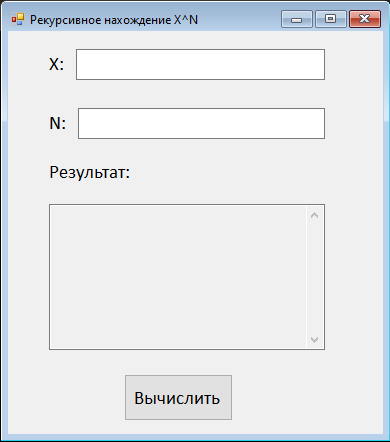
\includegraphics[width = 0.4\textwidth]{images/Task3/FormInConstructor.png}
    \caption{Вид формы в конструкторе}
    \label{fig:FormInConstruct3}
\end{figure}

\newpage

\subsection{Таблица с описанием переименовнных элементов формы}

Все элементы формы были переименованы и их атрибыты изменены. Проведенные изменения представлены в таблице \ref{tab:label3}

\begin{longtable}[!h]{|l|l|l|}
    \hline
    \makecell{$\textbf{Описание элементов}$\\ $\textbf{формы}$}& \makecell{$\textbf{Список измененных}$\\ $\textbf{атрибутов}$}& \makecell{$\textbf{Новое значение}$\\ $\textbf{атрибута}$}\\ 
    \hline
    \makecell{Форма}& \makecell{Text}& \makecell{Рекурсивные\\  вычисления $X^N$}\\ 
    \hline
    \makecell{Первая надпись (label)}& \makecell{Name}& \makecell{lblX}\\ 
    \hline
    \makecell{Первая надпись (label)}& \makecell{Text}& \makecell{X:}\\ 
    \hline
    \makecell{Вторая надпись (label)}& \makecell{Name}& \makecell{lblN}\\ 
    \hline
    \makecell{Вторая надпись (label)}& \makecell{Text}& \makecell{N:}\\ 
    \hline
    \makecell{Третья надпись (label)}& \makecell{Name}& \makecell{lblResult}\\ 
    \hline
    \makecell{Третья надпись (label)}& \makecell{Text}& \makecell{Результат:}\\ 
    \hline

    \makecell{Первое текстовое поле (textBox)}& \makecell{Name}& \makecell{txtInX}\\ 
    \hline
    \makecell{Второе текстовое поле (textBox)}& \makecell{Name}& \makecell{txtInY}\\ 
    \hline
    \makecell{Третье текстовое поле (textBox)}& \makecell{Name}& \makecell{txtOut}\\ 
    \hline
    \makecell{Третье текстовое поле (textBox)}& \makecell{ReadOnly}& \makecell{True}\\ 
    \hline
    \makecell{Кнопка (button)}& \makecell{Name}& \makecell{btnStart}\\ 
    \hline
    \makecell{Кнопка (button)}& \makecell{Text}& \makecell{Вычислить}\\ 
    \hline
    \makecell{Обработчик ошибок 1\\ (errorProvider)}& \makecell{Name}& \makecell{errPrX}\\ 
    \hline
    \makecell{Обработчик ошибок 2\\ (errorProvider)}& \makecell{Name}& \makecell{errPrN}\\ 
    \hline
    \caption{Значения атрибутов элементов в приложении <<Рекурсивные вычисления>>}
    \label{tab:label3}
\end{longtable}

\subsection{Примеры работы}

При запуске приложения на экране появляется окно (\ref{fig:StartForm3}).

\begin{figure}[!h]
    \centering
    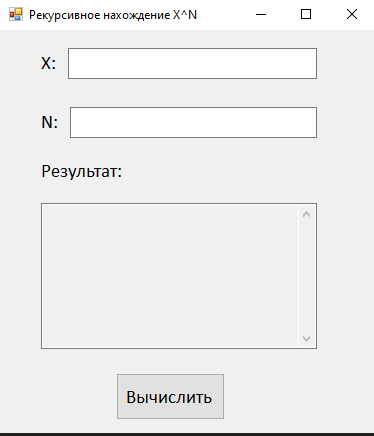
\includegraphics[width = 0.4\textwidth]{images/Task3/Start.png}
    \caption{Запуск приложения}
    \label{fig:StartForm3}
\end{figure}

При запуске с корректными данными (\ref{fig:WorkForm3})

\begin{figure}[!h]
    \centering
    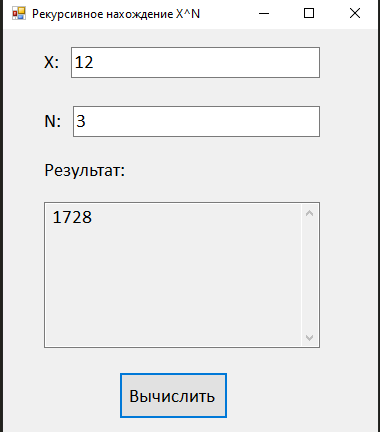
\includegraphics[width = 0.35\textwidth]{images/Task3/Work1.png}
    \caption{Запуск с корректными данными}
    \label{fig:WorkForm3}
\end{figure}

При запуске с некорректными данными (\ref{fig:BadInputNotIntForm3})

\begin{figure}[!h]
    \centering
    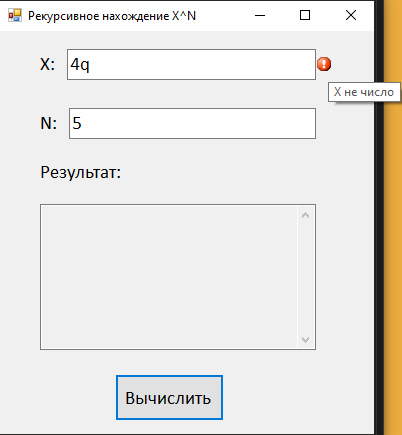
\includegraphics[width = 0.4\textwidth]{images/Task3/BadInputNotInt1.png}
    \caption{Запуск с некорректными данными}
    \label{fig:BadInputNotIntForm3}
\end{figure}

\subsection{Примеры кода}

Функция рекурсивно вычисляющая $x^n$:

\begin{minted}{c++}
// Функция рекурсивно вычисляющая x^n
double recursion(double x, long long n) {
	// если n == 0
	if (n == 0) {
		// то возвращаем 1
		return 1;
	}
	// если n > 0
	else if (n > 0) {
		// то возвращаем x * x^(n-1)
		return x * recursion(x, n - 1);
	}
	// если n < 0
	else {
		// то возвращаем 1 / (x^|n|)
		return 1 / recursion(x, abs(n));
	}
}
\end{minted}

Другие фрагменты кода расположены в приложении \ref{app:task3}. Полный код программы приведен в приложении \ref{app:zip}
